\documentclass[11pt,oneside,a4paper]{report}
\usepackage{amsmath}
\usepackage{booktabs}
\usepackage{graphicx}
\everymath{\displaystyle}
\setlength\parindent{0pt}
\begin{document}

\title{Project2 Report}

\author{Ye Feiyang \and Li Jianliang \and Yuan Xiaojie}

\date{July 25, 2012}

\maketitle

\section*{Introduction}

What is MAC protocol?\\
In this project, we will simulate four MAC protocals including ALOHA, Slotted ALOHA, CSMA and CSMA/CD. For each protocal, the basic thoeries will be introduced first, then several assumptions that clarify ...

\section*{Pure ALOHA}

\subsection*{Theories}

ALOHA was devised by Norman Abramson in the 1970s to solve the channel allocation problem. The basic idea of pure ALOHA is that users(or stations) can transimit frames whenever they have, which is totally random. Of course, when different users are transmiting their frames at the same time, those frames will collide and all of them will be damaged. A sender can find out whether its transmission succeed by checking the acknowledgements from the receiver. If the frame was damadged, it waits for a random time and send again. \\

Given the following parameters: \\

\qquad	\(X\): frame transmission time \\

\qquad	\(N\): average \# of frames genereted per frame time \\

\qquad	\(G\): load, average \# of transmission attempts per frame time \\

\qquad	\(k\): \# of transmissions attempts per frame time \\

\qquad	\(P\): probablity of a successful frame transmission \\

\qquad	\(S\): throughput, average \# of successful frames per frame time \\

We can derive that the probability that \(k\) frames are generated during a frame time \(X\) is given by the Poisson distribution \\

\qquad	\(P(k) = \frac{G^ke^{-G}}{k!}\) \\

So the probability of zero frames during the \(2G\) vulnerable time is \\

\qquad \(P(0)|_{G=2G} = e^{-2G}\) \\

Then the throughput is given by \\

\qquad \(S = Ge^{-2G}\) \\

for which the maximum occurs at \(G = 0.5\) with \(S = 1/2e \approx 0.184\) and the \(S - G\) graph is shown on Figure 1. \\

%\begin{figure}
%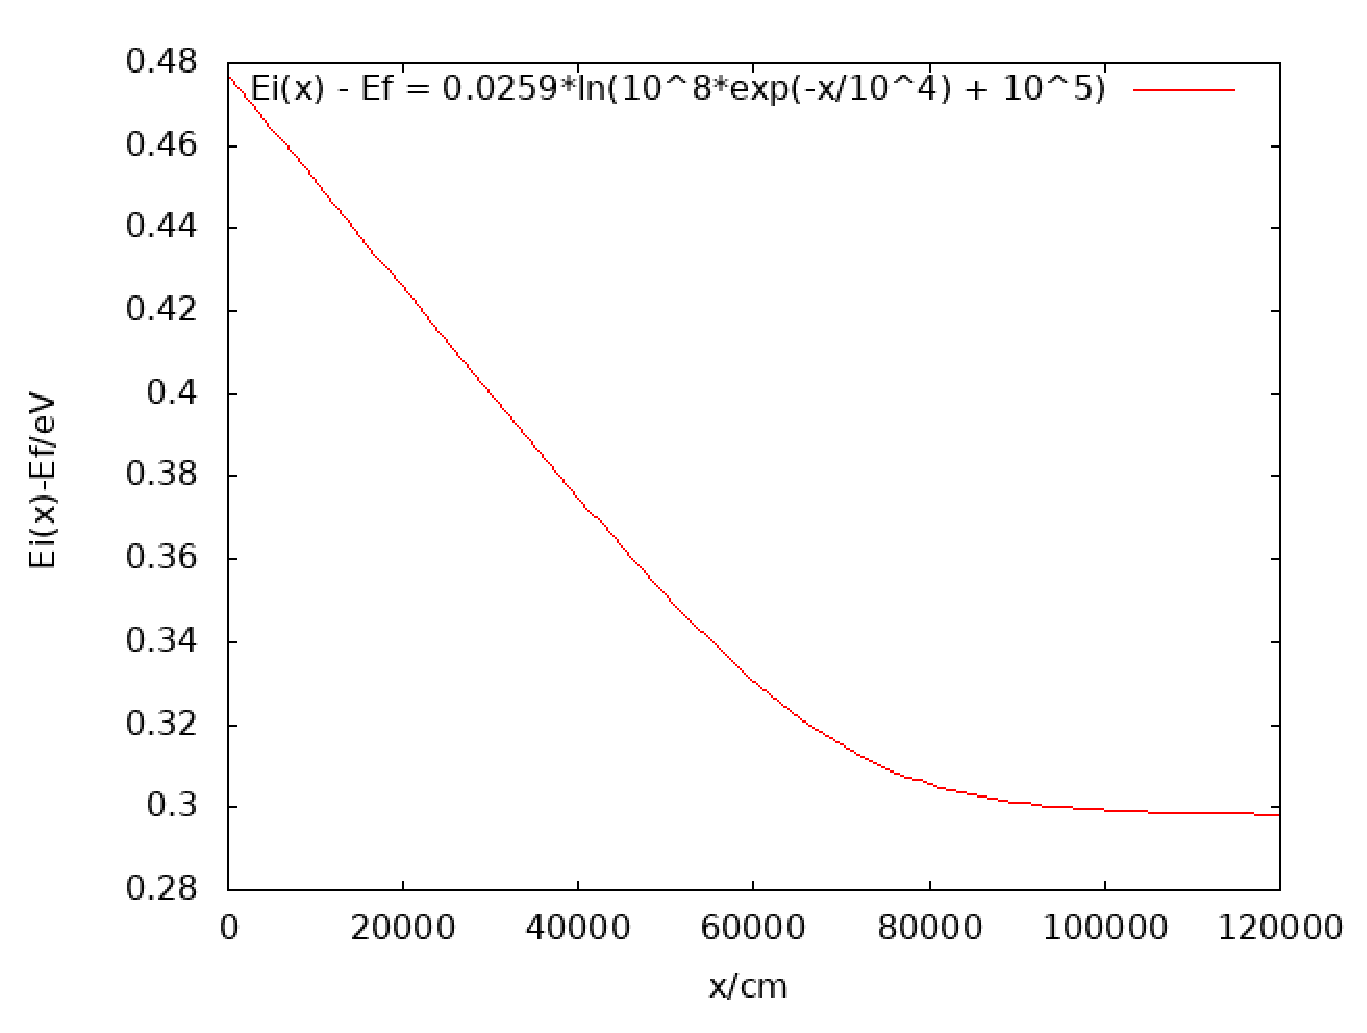
\includegraphics{1.eps}
%\caption{ALOHA}
%\end{figure}

\subsection*{Assumptions}

1. The length of each frame remains the same. \\
2. There is no propagation delay which means that one user can know whether its frames transmission succeed as soon as it finished its transimission. \\
3. The probability of an arrival during a short time interval \(\Delta t\) is propotional to the length of interval, and does not depend on the origin of the interval. \\
4. The probability of having multiple(\(>\) 1) arrivals during a short time interval \(\Delta t\) approaches 0; \\

\subsection*{Simulation}

In the simulation program, an two-dimensional array containing 0s and 1s is used to represent states of different users at each short time interval \(\Delta t\). For example, statest[\emph{userNum}][\emph{slotNum}] is an \emph{userNum}\(\times\)\emph{slotNum} array, its Nth(0 \(<\) N \(<\) \emph{userNum}) row represents that the Nth user's states from 0th to (\emph{slotNum}-1)th short time interval. "0" is used when the user is not transmitting data at a certain short time interval and "1" is used otherwise. \\

The array can be expressed graphically like this: \\

states[\emph{N}][\emph{M}]: \\

\qquad user1: 111111000111111\(\cdots\)0000000001111110000000 \\

\qquad user2: 001111110000000\(\cdots\)0001111110000000000111 \\

\qquad\quad \(\vdots\) \hspace{35mm} \(\vdots\) \\

\qquad userN: \hspace{-0.5mm}000000011111100\(\cdots\)1111110000001111110000 \\

Since the frame length(frameLen) is assumed to be constant, the number of consetutive 1s remains the same(except the frames at the end of each row). The above example always has 6 consetutive 1s which represents a 6-slot length frame. \\

At the beginnig of each simulation, the array need to be initialized based on a given probability \(p\) which is the probability that a user generates a frame during a certain short time interval \(\Delta t\). Once the first state is initialized to be 1, its consetutive (frameLen - 1) states should all be set to 1.\\

\subsection*{Results}

\subsection*{Analysis}

\section*{Slotted ALOHA}

\subsection*{Theories}

Slotted ALOHA is an advanced version of pure ALOHA. It divides time into descrete slots that each frame can only be sent at the beginning of each time slot. Moreover, slotted ALOHA requires global time synchronization so that the same slot boundaries can be agreed by all the users.

The vulnerable time for slotted ALOHA is half of the one for pure ALOHA. So the probability of zero frames during the G vulnerable time is \\

\qquad \(P(0)|_{G=G} = e^{-G}\) \\

Then the throughput is given by \\

\qquad \(S = Ge^{-G}\) \\

for which the maximum occurs at \(G = 1\) with \(S = 1/e \approx 0.368\) and the \(S - G\) graph is shown on Figure 1.

\subsection*{Assumptions}

\subsection*{Simulation}

\subsection*{Results}

\subsection*{Analysis}

\section*{CSMA}

\section*{CSMA/CD}

\end{document}

